%%
%% This is file `sample-sigconf.tex',
%% generated with the docstrip utility.
%%
%% The original source files were:
%%
%% samples.dtx  (with options: `sigconf')
%% 
%% IMPORTANT NOTICE:
%% 
%% For the copyright see the source file.
%% 
%% Any modified versions of this file must be renamed
%% with new filenames distinct from sample-sigconf.tex.
%% 
%% For distribution of the original source see the terms
%% for copying and modification in the file samples.dtx.
%% 
%% This generated file may be distributed as long as the
%% original source files, as listed above, are part of the
%% same distribution. (The sources need not necessarily be
%% in the same archive or directory.)
%%
%%
%% Commands for TeXCount
%TC:macro \cite [option:text,text]
%TC:macro \citep [option:text,text]
%TC:macro \citet [option:text,text]
%TC:envir table 0 1
%TC:envir table* 0 1
%TC:envir tabular [ignore] word
%TC:envir displaymath 0 word
%TC:envir math 0 word
%TC:envir comment 0 0
%%
%%
%% The first command in your LaTeX source must be the \documentclass command.
\documentclass[sigconf,review]{acmart}
%\documentclass[sigconf]{acmart}

\usepackage{pxfonts}
\usepackage[scaled]{helvet}
\usepackage{url}
%\usepackage[dvipsnames]{xcolor}
\usepackage{hyperref}
\hypersetup{
  colorlinks=true,
  allcolors=NavyBlue
}
\usepackage{graphicx}
\usepackage[utf8]{inputenc}
\usepackage{caption}
\usepackage{subcaption}
\usepackage{listings}
\usepackage{longtable}
\usepackage[export]{adjustbox}
%\lstset{
  %  basicstyle=\footnotesize\ttfamily
  %}
\lstset{
  basicstyle=\ttfamily,
  frame=none,
  breaklines=true,
  numbers=left,
  xleftmargin=2.5em,
  framexleftmargin=0em,
  emphstyle=\textbf,
  float=t
  %  ,escapeinside={/*}{*/}
  ,moredelim=[is][\bfseries]{(*}{*)}
}
\lstdefinestyle{egx}{
  basicstyle=\ttfamily\scriptsize,
  emph={
    rule, transform, template, parameters, Map, Sequence, :
  },
  commentstyle=\sffamily\textit,
  comment=[l]{\#}
}
\lstdefinestyle{egl}{
  basicstyle=\ttfamily\scriptsize
}
\lstdefinestyle{model}{
  basicstyle=\ttfamily\scriptsize,
  emph={
    <, ?, xml, SocialNetwork, >, xmi, :, id, name, =, likes, dislikes, /,
    people, encoding, version, xmlns
  },
}
\lstdefinestyle{picto}{
  basicstyle=\ttfamily\scriptsize,
  emph={
    <, ?, /, :, >, =,
    nsuri, picto, format, icon, view, path, parameter, values,
    name, format, position, source, transformation, type
  },
}

\hyphenation{
  File-Watch-er Trans-form-er View-Con-tent-Cache Pic-to-Con-trol-ler
}


%%
%% \BibTeX command to typeset BibTeX logo in the docs
\AtBeginDocument{%
  \providecommand\BibTeX{{%
    \normalfont B\kern-0.5em{\scshape i\kern-0.25em b}\kern-0.8em\TeX}}}

%% Rights management information.  This information is sent to you
%% when you complete the rights form.  These commands have SAMPLE
%% values in them; it is your responsibility as an author to replace
%% the commands and values with those provided to you when you
%% complete the rights form.
\setcopyright{acmcopyright}
\copyrightyear{2022}
\acmYear{2022}
\acmDOI{XXXXXXX.XXXXXXX}

%% These commands are for a PROCEEDINGS abstract or paper.
\acmConference[MODELS '22]{Make sure to enter the correct
  conference title from your rights confirmation emai}{October 23--28,
  2022}{Montreal, Canada}
\acmPrice{15.00}
\acmISBN{978-1-4503-XXXX-X/22/10}


%%
%% Submission ID.
%% Use this when submitting an article to a sponsored event. You'll
%% receive a unique submission ID from the organizers
%% of the event, and this ID should be used as the parameter to this command.
%%\acmSubmissionID{123-A56-BU3}

%%
%% The majority of ACM publications use numbered citations and
%% references.  The command \citestyle{authoryear} switches to the
%% "author year" style.
%%
%% If you are preparing content for an event
%% sponsored by ACM SIGGRAPH, you must use the "author year" style of
%% citations and references.
%% Uncommenting
%% the next command will enable that style.
%%\citestyle{acmauthoryear}

%%
%% end of the preamble, start of the body of the document source.
\begin{document}

%%
%% The "title" command has an optional parameter,
%% allowing the author to define a "short title" to be used in page headers.
\title{Picto Web: A Tool for Complex Model Exploration}

%%
%% The "author" command and its associated commands are used to define
%% the authors and their affiliations.
%% Of note is the shared affiliation of the first two authors, and the
%% "authornote" and "authornotemark" commands
%% used to denote shared contribution to the research.
%\author{Ben Trovato}
%\authornote{Both authors contributed equally to this research.}
%\email{trovato@corporation.com}
%\orcid{1234-5678-9012}
%\author{G.K.M. Tobin}
%\authornotemark[1]
%\email{webmaster@marysville-ohio.com}
%\affiliation{%
%  \institution{Institute for Clarity in Documentation}
%  \streetaddress{P.O. Box 1212}
%  \city{Dublin}
%  \state{Ohio}
%  \country{USA}
%  \postcode{43017-6221}
%}
%
%\author{Lars Th{\o}rv{\"a}ld}
%\affiliation{%
%  \institution{The Th{\o}rv{\"a}ld Group}
%  \streetaddress{1 Th{\o}rv{\"a}ld Circle}
%  \city{Hekla}
%  \country{Iceland}}
%\email{larst@affiliation.org}
%
%\author{Valerie B\'eranger}
%\affiliation{%
%  \institution{Inria Paris-Rocquencourt}
%  \city{Rocquencourt}
%  \country{France}
%}
%
%\author{Aparna Patel}
%\affiliation{%
% \institution{Rajiv Gandhi University}
% \streetaddress{Rono-Hills}
% \city{Doimukh}
% \state{Arunachal Pradesh}
% \country{India}}

\author{Alfa Yohannis}
\affiliation{%
  \institution{University of York}
%  \streetaddress{30 Shuangqing Rd}
  \city{York}
  \state{North Yorkshire}
  \country{United Kingdom}}
\email{alfa.yohannis@york.ac.uk}

\author{Dimitris Kolovos}
\affiliation{%
  \institution{University of York}
  %  \streetaddress{30 Shuangqing Rd}
  \city{York}
  \state{North Yorkshire}
  \country{United Kingdom}}
\email{dimitris.kolovos@york.ac.uk}

%\author{Charles Palmer}
%\affiliation{%
%  \institution{Palmer Research Laboratories}
%  \streetaddress{8600 Datapoint Drive}
%  \city{San Antonio}
%  \state{Texas}
%  \country{USA}
%  \postcode{78229}}
%\email{cpalmer@prl.com}
%
%\author{John Smith}
%\affiliation{%
%  \institution{The Th{\o}rv{\"a}ld Group}
%  \streetaddress{1 Th{\o}rv{\"a}ld Circle}
%  \city{Hekla}
%  \country{Iceland}}
%\email{jsmith@affiliation.org}
%
%\author{Julius P. Kumquat}
%\affiliation{%
%  \institution{The Kumquat Consortium}
%  \city{New York}
%  \country{USA}}
%\email{jpkumquat@consortium.net}

%%
%% By default, the full list of authors will be used in the page
%% headers. Often, this list is too long, and will overlap
%% other information printed in the page headers. This command allows
%% the author to define a more concise list
%% of authors' names for this purpose.
\renewcommand{\shortauthors}{Yohannis, et al.}

%%
%% The abstract is a short summary of the work to be presented in the
%% article.
\begin{abstract}
  A clear and well-documented \LaTeX\ document is presented as an
  article formatted for publication by ACM in a conference proceedings
  or journal publication. Based on the ``acmart'' document class, this
  article presents and explains many of the common variations, as well
  as many of the formatting elements an author may use in the
  preparation of the documentation of their work.
\end{abstract}

%%
%% The code below is generated by the tool at http://dl.acm.org/ccs.cfm.
%% Please copy and paste the code instead of the example below.
%%
\begin{CCSXML}
	<ccs2012>
	<concept>
	<concept_id>10011007.10011006.10011066.10011069</concept_id>
	<concept_desc>Software and its engineering~Integrated and visual development environments</concept_desc>
	<concept_significance>300</concept_significance>
	</concept>
	<concept>
	<concept_id>10003120.10003145.10003147.10010365</concept_id>
	<concept_desc>Human-centered computing~Visual analytics</concept_desc>
	<concept_significance>300</concept_significance>
	</concept>
	<concept>
	<concept_id>10003120.10003145.10003151.10011771</concept_id>
	<concept_desc>Human-centered computing~Visualization toolkits</concept_desc>
	<concept_significance>300</concept_significance>
	</concept>
	<concept>
	<concept_id>10011007.10011006.10011050.10011017</concept_id>
	<concept_desc>Software and its engineering~Domain specific languages</concept_desc>
	<concept_significance>300</concept_significance>
	</concept>
	</ccs2012>
\end{CCSXML}

\ccsdesc[300]{Software and its engineering~Integrated and visual development environments}
\ccsdesc[300]{Human-centered computing~Visual analytics}
\ccsdesc[300]{Human-centered computing~Visualization toolkits}
\ccsdesc[300]{Software and its engineering~Domain specific languages}

%%
%% Keywords. The author(s) should pick words that accurately describe
%% the work being presented. Separate the keywords with commas.
\keywords{complex models, model exploration, picto, web, visualisation}

%%% A "teaser" image appears between the author and affiliation
%%% information and the body of the document, and typically spans the
%%% page.
%\begin{teaserfigure}
%  \includegraphics[width=\textwidth]{sampleteaser}
%  \caption{Seattle Mariners at Spring Training, 2010.}
%  \Description{Enjoying the baseball game from the third-base
%  seats. Ichiro Suzuki preparing to bat.}
%  \label{fig:teaser}
%\end{teaserfigure}

%%
%% This command processes the author and affiliation and title
%% information and builds the first part of the formatted document.
\maketitle

\section{Introduction}
\label{sec:introduction}
A model is commonly considered complex when it has a large number of heterogeneous elements which are involved in non-trivial relationships \cite{boccara2010complex,klosterman2012complex}. One way to understand and communicate such models is through visualisation. However, displaying all elements and their relationships in a single graphical representation is often undesirable since it can overload users with information and make visualisations challenging to comprehend. In terms of computation, this approach is also inefficient for large models since a potentially very large and complex diagram has to be rendered in one go. Thus, novel mechanisms are necessary to allow engineers and other stakeholders to perform contextual exploration of complex models from different viewpoints and at different levels of detail. 

In this report, we present Picto Web, a web-based version of the Picto\footnote{\url{https://www.eclipse.org/epsilon/doc/picto}} \cite{dimitris2020picto} model visualisation tool which was originally implemented as an extension of the Eclipse IDE. Unlike Picto, Picto Web does not require local software installation, which makes it more suitable for a broader audience of developers and stakeholders who would benefit from access to dynamically-generated graphical views of complex software and system models.


\section{Picto}
\label{sec:picto}

Earlier in our work we developed Picto \cite{dimitris2020picto}, an Eclipse plugin that uses lazy model-to-text transformation to generate transient graphical views from heterogeneous models. Figure \ref{fig:picto-eclipse} shows a screenshot of Picto for Eclipse.

In the example of Figure \ref{fig:picto-eclipse}, we wish to visualise models conforming to a contrived social network metamodel from \cite{dimitris2020picto}. In particular, we use a sample model containing four persons (Alice, Bob,  Charlie and Dawn) and like/dislike relationships between them. From such social network models we wish to produce one node-edge view for the entire social network, and one view for each member of the network that omits any persons they neither like nor dislike. 

Picto’s user interface has two main components. On its left-hand side is a tree widget that displays the titles and icons of the views (Social Network, Alice, Bob, Charlie and Dawn) that users can select from. Once a view is selected, its content is generated and rendered in an embedded web browser -- through a series of transformations -- on the right-hand side of Picto. In Figure \ref{fig:picto-eclipse}, the selected view visualises the entire model in the form of a Graphviz-based node-edge diagram. Beyond Graphviz, Picto also supports PlantUML and SVG/HTML as visualisation formats, and also features an extensible architecture that enables adopters to extend it with additional diagram-as-code formats.  

\begin{figure}[h]
  \centering
  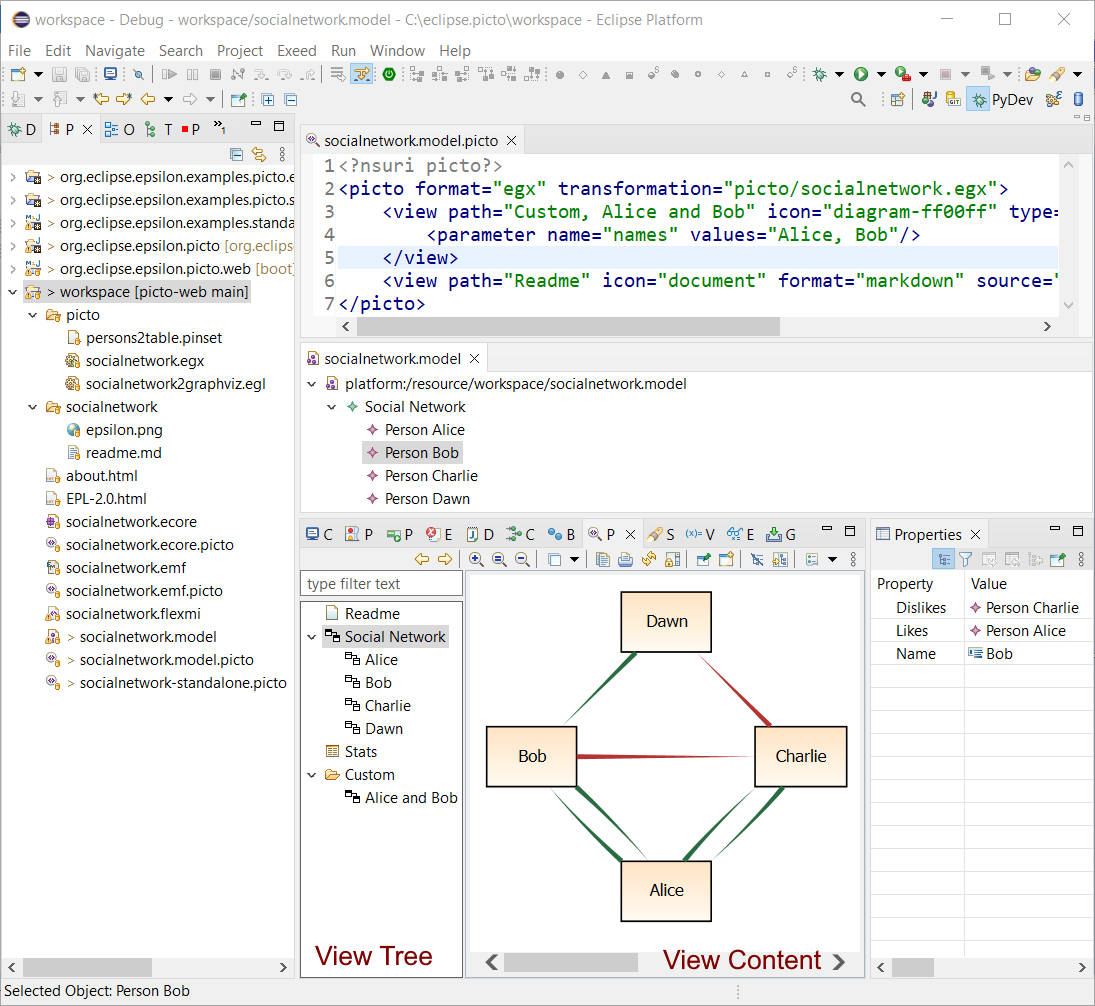
\includegraphics[width=\linewidth]{images/picto-eclipse.png}
  \caption{Picto plugin for Eclipse environment.}
  \label{fig:picto-eclipse}
\end{figure}

A challenge with Picto is that it is implemented as a plugin of the Eclipse IDE, which means that for engineers to use it, they need to install Java, Eclipse and Picto and check out the models they wish to explore (as well as the respective visualisation transformations) locally. While this is not an issue for software developers who are already familiar with Eclipse, it can represent a significant barrier for other engineers and stakeholders. When we first introduced Picto to our partners, there was a strong interest for an Eclipse-independent version of the tool which would be accessible through a standard web browser with no further local software installation requirements. This motivated us to develop Picto Web, which is presented below.

\section{Picto Web}

Picto Web\footnote{\url{https://github.com/alfayohannis/picto-web}} is a web-based version of Picto. 
It maintains the core features of the desktop version of Picto, such as supporting the lazy generation of views, drilling-up/down tree views, multi-views, and multi-formats, but it is implemented as a multi-tenant client-server web application that can be accessed through a standard web browser to perform interactive complex model exploration. 
Picto Web monitors model files and visualisation templates for changes and immediately propagates the modification to the viewers' web browsers, delivering a live user experience.

\subsection{Running Example}
\label{sec:running_example}

This report uses the same contrived social network example as in the original Picto documentation\footnote{\url{https://eclipse.org/epsilon/doc/picto}} to explain Picto Web. As a brief refresher, a social network is a graph that contains a number of people as its nodes linked with \emph{like} and \emph{dislike} relationships. In a view, as shown in Figure \ref{fig:ui_social_network}, a person is depicted as a rectangle while the \emph{like} and \emph{dislike} relationships are presented as green and red edges respectively. This node-edge view is the visualisation of the social network model defined in Listing \ref{lst:model}.

\subsection{User Interface}
\label{sec:user_interface}

\begin{figure*}[h]
  \centering
  \hfill
  \begin{subfigure}{0.49\textwidth}
    \frame{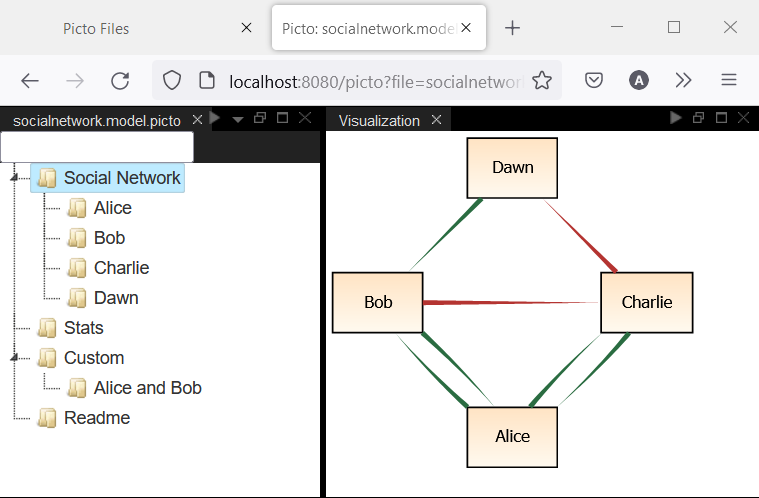
\includegraphics[width=\textwidth]{images/gui-social-network.png}}
    \caption{the overall social network}
    \label{fig:ui_social_network}
  \end{subfigure}
  \hfill
  \begin{subfigure}{0.49\textwidth}
    \frame{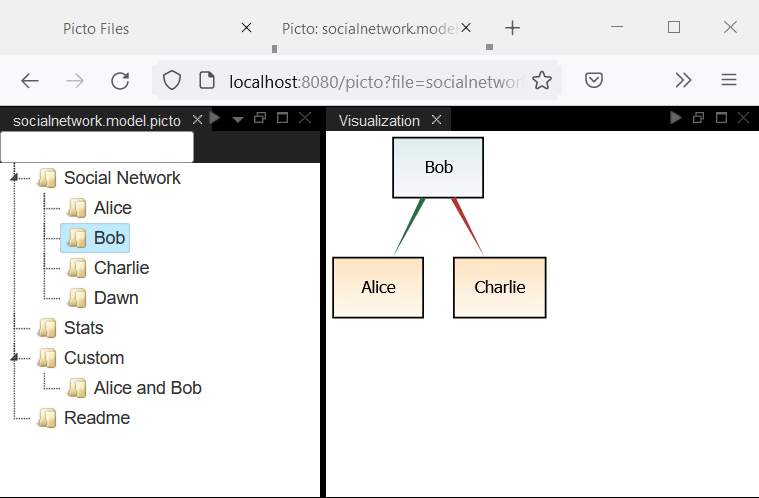
\includegraphics[width=\textwidth]{images/gui-bob.png}}
    \caption{Bob's social network}
    \label{fig:ui_bob}
  \end{subfigure}
  \hfill
  \begin{subfigure}{0.49\textwidth}
    \frame{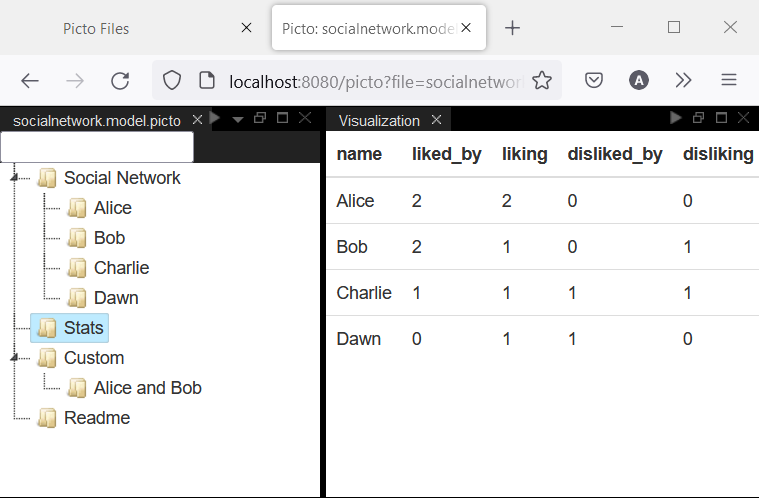
\includegraphics[width=\textwidth]{images/gui-tabular.png}}
    \caption{a HTML table summarising the social network}
    \label{fig:ui_tabular}
  \end{subfigure}
  \hfill
  \begin{subfigure}{0.49\textwidth}
    \frame{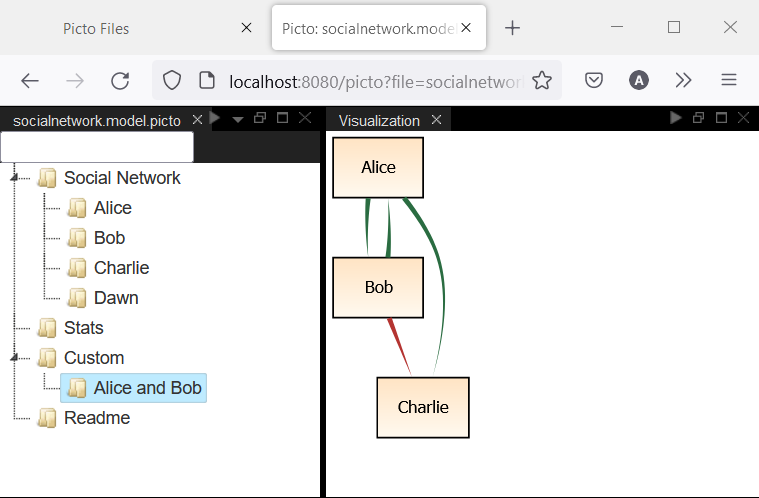
\includegraphics[width=\textwidth]{images/gui-custom.png}}
    \caption{custom Alice and Bob's social network}
    \label{fig:ui_custom}
  \end{subfigure}
  \hfill
  \caption{Picto Web client displays different views.}
  \label{fig:ui}
\end{figure*}

Figure \ref{fig:ui} shows the user interface (UI) of Picto Web. The UI has two main areas. The left side is a tree view which lists the views produced from the underpinning model(s) in a hierarchical way, and the right side is a panel that displays the content of the active, selected view. In our example, when a user selects the \emph{Social Network} view on the left hand side, Picto Web displays the overall social network of Alice, Bob, Charlie, and Dawn (Figure \ref{fig:ui_social_network}). 

Viewers can also drill down to display the local social network of each person through the tree view on the left. For example, Figure \ref{fig:ui_bob} displays Bob's social network. Besides being able to display view contents in SVG/HTML as in Figures \ref{fig:ui_social_network} and \ref{fig:ui_bob}, Picto Web is also able to render model views in other formats. For example, Figure \ref{fig:ui_tabular} displays a summary of the social network in the form of a HTML table. 

In addition to procedurally-generated views (e.g. one view for each person in the network), developers can also define custom views, as shown in Figure \ref{fig:ui_custom}. The figure displays the social network of Alice and Bob and is explicitly defined as a \emph{view} element in lines 3-5 of the Picto file in Listing \ref{lst:picto}.

\subsection{Transformation}
\label{sec:transformation}

Picto requires at least three types of files: model files (any model representation format supported by Epsilon\footnote{\url{https://eclipse.org/epsilon/doc/emc}} is also supported by Picto Web), visualisation transformation files in Epsilon's EGL template-based language (*.egx, *.egl), and Picto files (*.picto) which bind models to visualisation transformations and specify custom views. Listing \ref{lst:model} shows the XMI-based representation of the social network model of our running example. 

\begin{lstlisting}[firstnumber=1,style=model,caption={An a social network model as the input file for the lazy transformation. The format of the ids is simplified.},label=lst:model]
<?xml version="1.0" encoding="ASCII"?>
  <SocialNetwork xmlns="socialnetwork" xmi:id="sn">
  <people xmi:id="a" name="Alice" likes="b c"/>
  <people xmi:id="b" name="Bob" likes="a" dislikes="c"/>
  <people xmi:id="c" name="Charlie" likes="a" dislikes="d"/>
  <people xmi:id="d" name="Dawn" likes="b"/>
</SocialNetwork>
\end{lstlisting}

The EGL transformation files consist of EGL templates that produce individual views, and an EGX coordination program that specifies how the templates should be executed against different elements in the mode(s). Listing \ref{lst:egx} shows an excerpt of the EGX transformation coordination program of this example. Rule \texttt{Network2Graphviz} runs the \texttt{socialnetwork2} \texttt{graphviz.egl} template of Listing \ref{lst:egl} for every \texttt{SocialNetwork} element in the source model and produces a Graphviz-based view for it. The EGL template of Listing \ref{lst:egl} defines the logic for generating the content of the view. An actual generated view in Graphviz is shown in Listing \ref{lst:output}. 

\begin{lstlisting}[firstnumber=1,style=egx,caption={The Network2Graphviz EGX rule},label=lst:egx]
rule Network2Graphviz 
  transform n : socialnetwork::SocialNetwork {
  template : "socialnetwork2graphviz.egl"
  parameters : Map{
    "path" = Sequence{"Social Network"},
    "format" = "graphviz-circo",
    "people" = n.people
  }
}
\end{lstlisting}


\begin{lstlisting}[firstnumber=1,style=egx,caption={An EGL template that generates a Graphviz representation of a social network.},label=lst:egl]
digraph G {
  node[shape=rectangle, fontname=Tahoma, fontsize=10, style="filled", gradientangle="270", fillcolor="bisque:floralwhite"]
  edge[penwidth=3, style=tapered, arrowhead=none]
  (*[%for (p in people){%]*)
    (*[%=p.name%]*)
    (*[%for (l in p.likes){%]*)
      (*[%=p.name%] -> [%=l.name%]*) [color=green]
    (*[%}%]*)
    (*[%for (l in p.dislikes){%]*)
      (*[%=p.name%] -> [%=l.name%]*) [color=red]
    (*[%}%]*)
  (*[%}%]*)
}
\end{lstlisting}

\begin{lstlisting}[firstnumber=1,style=egx,caption={A view generated by the EGL template in Listing \ref{lst:egl}.},label=lst:output]
digraph G {
  node[shape=rectangle, fontname=Tahoma, fontsize=10, style="filled", gradientangle="270", fillcolor="bisque:floralwhite"]
  ...
  Alice
  Alice -> Bob [color=green]
  ...
  Dawn
  Dawn -> Bob [color=green] 
}
\end{lstlisting}

Picto files bind the transformation coordination and model files to generate the contents of the target views. In Listing \ref{lst:picto}, Picto Web uses the \texttt{socialnetwork.egx} transformation coordination file that contains the rule in Listing \ref{lst:egx} to transform the social network model in Listing \ref{lst:model} into the social network and individual person views shown in Figure \ref{fig:ui}. It also includes two additional views: (1) a custom view that includes only Alice and Bob's social network (Figure \ref{fig:ui_custom}) and (2) a view that displays a Markdown readme file.

\begin{lstlisting}[firstnumber=1,style=picto,caption={The Picto file that binds the model and the visualisation transformation.},label=lst:picto]
<?nsuri picto?>
  <picto format="egx" transformation="picto/socialnetwork.egx">
    <view path="Custom, Alice and Bob" icon="diagram-ff00ff" type="Persons2Graphviz">
      <parameter name="names" values="Alice, Bob"/>
    </view>        
    <view path="Readme" icon="document" format="markdown" source="socialnetwork/readme.md" position="0"/>
</picto>
\end{lstlisting}


\subsection{Architecture}
\label{sec:architecture}

The architecture of Picto Web is displayed in Figure \ref{fig:architecture} and consists of two parts: a server-side part that lazily runs visualisation transformations against models, and a browser-based client that displays the visualisation results. 

%one that runs in the local modelling environment and the other one in the remote environment. 
%The latter is the Picto Web client, a web client application that runs on viewers' web browsers and is used to navigate complex models. 
%The former is the environment dedicated for modellers to construct models and consists of, minimum, a model editor, the models under construction, and a Picto Web server application. 

\begin{figure}[h]
  \centering
  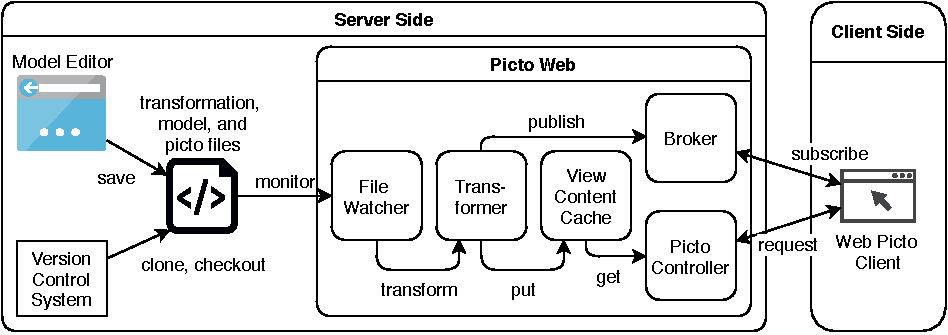
\includegraphics[width=\linewidth]{images/architecture.pdf}
  \caption{The architecture of Picto Web.}
  \label{fig:architecture}
\end{figure}

The server-side part is composed of the \texttt{FileWatcher}, \texttt{Transformer}, \texttt{ViewContentCache}, \texttt{PictoController}, and \texttt{Broker} components shown on the left hand side of the figure. The \texttt{FileWatcher} component is responsible for monitoring a directory that contains the models that Picto Web needs to visualise (see Section \ref{sec:picto}). When any of the files is modified (added, deleted, or updated), \texttt{FileWatcher} detects the change and notifies the \texttt{Transformer} component, which then generates, refreshes, or invalidates the contents of the respective views. 

After that, Picto Web puts the generated views into a cache (\texttt{ViewContentCache}) that maps the paths of the views in the tree view to their actual contents. The cache is used to avoid wastefully re-generating views which cannot have been impacted since the last time a client requested them.

Every time a client requests the content of a specific view, \texttt{PictoController} receives and handles the request by retrieving the view content from \texttt{ViewContentCache} using the view's path sent in the request as the key for the map. The retrieved content is then returned to the client to display.

\texttt{Broker} is a component responsible for pushing updates to Picto Web clients. Every time a Picto Web client starts visualising a model, the client subscribes to the \texttt{Broker} so that it can receive further updates from the Picto Web server-side component if any of the model files are subsequently modified. After transformation, the \texttt{Transformer} publishes new content views to the \texttt{Broker}.

We have packed the Picto Web server in the form of Docker image\footnote{\url{https://hub.docker.com/r/alfayohannisyorkacuk/picto-web}} so that users can easily deploy and test it. Users need to run the following command to launch the Docker image.\\\\ 
%
\texttt{docker run --rm -i -t -v \$PWD:/workspace --hostname=\\picto -p 8080:8080 --name=picto picto-web}\\\\
%
The Picto Web server can then be accessed using a web browser via \texttt{http://localhost:8080}. Note the \texttt{\$PWD:/workspace} virtual directory mapping argument that is used to map the current active directory \texttt{\$PWD} to  the Docker image's internal \texttt{/workspace} directory. The current active directory should contain Picto and all model and transformation files. This way, the internal \texttt{FileWatcher} in the Picto Web Docker image can monitor the file system for any relevant changes that should trigger view generation or invalidation.

\subsection{Control Flow}

\begin{figure}[h]
  \centering
  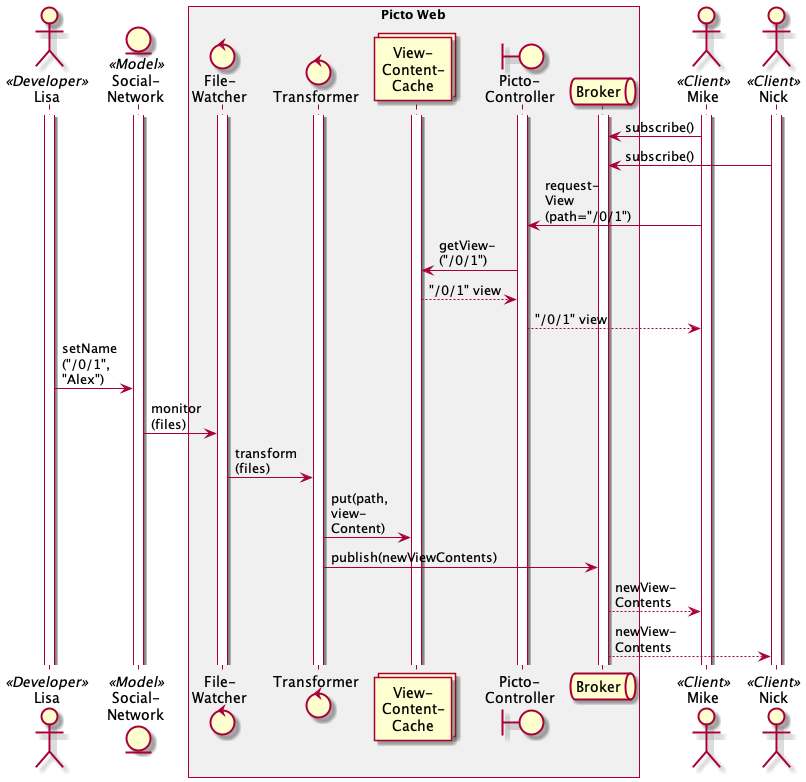
\includegraphics[width=0.89\linewidth]{images/sequence.png}
  \caption{Requests and Updates of Picto Web's view contents.}
  \label{fig:sequence}
\end{figure}

This section demonstrates Picto Web's internal control flow, visualised in the sequence diagram in Figure \ref{fig:sequence}. Suppose that the \texttt{ViewContentCache} has been populated with view contents through an initial transformation executed when a developer (Lisa) created the social network model---the process is not displayed in the diagram. Stakeholders Mike and Nick wish to explore Lisa's model and start running Picto Web clients. The clients subscribe to the broker provided by the Picto Web server application so that they can receive further updates on the model. 

Mike is interested in knowing more about Alice's social network. Therefore, he sends a view request to Picto Web with a parameter containing Alice's view path, ``/0/1''\footnote{Simplified format}. Since the view content of the path is already available in the \texttt{ViewContentCache} from the initial transformation, \texttt{PictoController}, the class that handles the request, retrieves Alice's view content from the cache and sends it back to Mike's client to be displayed.

At some point, Lisa decides to rename `Alice' to `Alex' and save the change to the model file. \texttt{FileWatcher} detects that the file has been modified and notifies the \texttt{Transformer} to generate new view contents from the modified file and update the \texttt{ViewContentCache}. The \texttt{Transformer} also publishes the new content views to the \texttt{Broker} so that the subscribers, Mike and Nick, also receive the new content views and perform live updates on the view contents they currently display.

\section{Related Work}
Sprotty \cite{sprotty2022git} is an open-source diagramming framework that uses web technologies to render graphical views. 
Besides being used on the client-side for fast, scalable SVG rendering with ELK layout, it also provides a headless component that can be used for integration with the Xtext framework, extending Language Server Protocol, and computing diagram layout on the server side. 

Sprotty only supports node-edge diagrams and does not support rendering views conforming to different technologies, such as tables in HTML, PlantUML and Graphviz diagrams. Moreover, Sprotty does not support semantic editing on diagrams. As an alternative, the Graphical Language Server Platform (GLSP) \cite{eclipse2022glsp} allows complete control and access over the Sprotty diagrams and can be considered if diagram editing via web browsers is required.

KIELER Lightweight Diagram (KLD) framework \cite{schneider2013just} uses XTend, Piccolo2D and EMF to allow on-demand model visualisation, and also the KIELER Infrastructure for Meta Layout (KIML) for defining diagram layouts. KLD uses three EMF-based models -- KLayoutData, KRendering, and KGraph -- for users to describe a diagram. KLD is also extensible via Java/Xtend interfaces, which should be implemented to transform and map a semantic model to KGraph and KRendering models. 

Similar to Sprotty, it only supports rendering views in node-edge diagrams. As a comparison, Picto and Picto Web support rendering views in multiple formats, such as table/form views in HTML, PlatUML and Graphviz diagrams, and views generated using JavaScript graphical libraries, e.g., Three.js.


\section{Conclusions and Future Work}
\label{sec:conclusions_and_future_work}

In this report, we presented Picto Web, a web-based version of the Picto model visualisation tool which was originally implemented as a plug-in of the Eclipse IDE. Unlike Picto, Picto Web does not require local software installation, which makes it more suitable for a broader audience of developers and stakeholders who would benefit from access to dynamically-generated graphical views of complex software and system models. Going forward, we plan to further improve the performance of visualisation transformations in Picto Web by establishing an element/property access trace of the visualisation transformations, to enable more fine-grained regeneration and invalidation of generated views.

%In this report, we have presented Picto Web, an extension of the Eclipse Picto plugin. We use web technologies to make Picto's complex model exploration accessible concurrently to multiple remote viewers and unbounded by the Eclipse environment. In the next phase, we plan to improve the performance of Picto Web by identifying the elements and properties accessed during a transformation. Therefore, we can optimise the performance by only (re)generating view contents associated with the accessed elements and properties instead of generating all view contents when a model file is modified. 



\bibliographystyle{ACM-Reference-Format}
\bibliography{bibliography}

\end{document}
\endinput
%%
%% End of file `sample-sigconf.tex'.
